\newpage
\section{Evaluation}
Para la valoración de la experiencia de usuario, se ha propuesto a 14 usuarios que prueben la herramienta libremente. 
Tras una semana, se propone a los usuarios de prueba una encuesta que contiene preguntas concretas sobre la comprensibilidad
de la información y sobre la usabilidad. Además, se les proporciona un espacio en cada una de las preguntas para que los
encuestados puedan realizar sus propias aportaciones. 

\begin{figure}[ht]
   \centering
   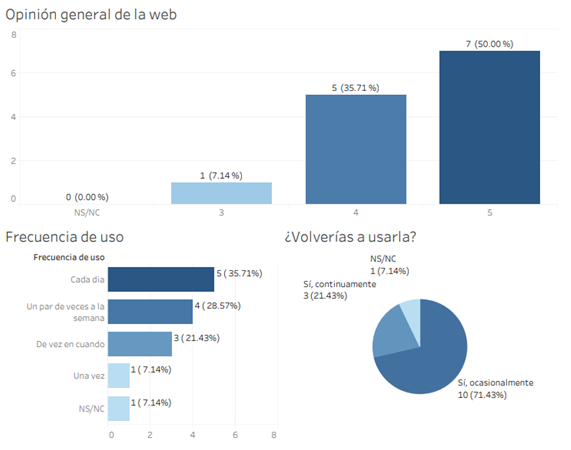
\includegraphics[width=12cm]{enqueteResults}
   \caption{Part of the user experience enquete results}
\end{figure}

En cuanto a los comentarios, la mayoría de los encuestados coinciden que la funcionalidad que más les ha gustado es ver en el 
mapa el índice de calidad del aire y sugieren una ampliación el número de zonas.
El 92\% de los encuestados encuentra la información útil y completa y el 71,43\% ha contestado que también la encuentran 
comprensible.
Más de la mitad de los encuestados admiten que no conocían el significado del índice de calidad del aire, pero después de 
consultar la ayuda, lo han entendido.
Respecto a sus intereses sobre la calidad del aire, la mitad de ellos indican que alguna vez han buscado información sobre ello, 
sólo dos están bien informados y uno de ellos marca la opción otros y especifica que ha despertado su interés después de utilizar 
la aplicación.
Además, cuatro de ellos indican que han descubierto que tienen una condición médica a la que le afecta la calidad del aire gracias 
a la herramienta.

Entre los sujetos de prueba, se ha reconocido una mayor concienciación por la contaminación, demostrando más interés sobre la 
calidad del aire en la ciudad y sus posibles efectos en la salud

